\documentclass[]{article}
\usepackage{lmodern}
\usepackage{amssymb,amsmath}
\usepackage{ifxetex,ifluatex}
\usepackage{fixltx2e} % provides \textsubscript
\ifnum 0\ifxetex 1\fi\ifluatex 1\fi=0 % if pdftex
  \usepackage[T1]{fontenc}
  \usepackage[utf8]{inputenc}
\else % if luatex or xelatex
  \ifxetex
    \usepackage{mathspec}
  \else
    \usepackage{fontspec}
  \fi
  \defaultfontfeatures{Ligatures=TeX,Scale=MatchLowercase}
\fi
% use upquote if available, for straight quotes in verbatim environments
\IfFileExists{upquote.sty}{\usepackage{upquote}}{}
% use microtype if available
\IfFileExists{microtype.sty}{%
\usepackage[]{microtype}
\UseMicrotypeSet[protrusion]{basicmath} % disable protrusion for tt fonts
}{}
\PassOptionsToPackage{hyphens}{url} % url is loaded by hyperref
\usepackage[unicode=true]{hyperref}
\hypersetup{
            pdfborder={0 0 0},
            breaklinks=true}
\urlstyle{same}  % don't use monospace font for urls
\usepackage[margin=1in]{geometry}
\usepackage{color}
\usepackage{fancyvrb}
\newcommand{\VerbBar}{|}
\newcommand{\VERB}{\Verb[commandchars=\\\{\}]}
\DefineVerbatimEnvironment{Highlighting}{Verbatim}{commandchars=\\\{\}}
% Add ',fontsize=\small' for more characters per line
\usepackage{framed}
\definecolor{shadecolor}{RGB}{248,248,248}
\newenvironment{Shaded}{\begin{snugshade}}{\end{snugshade}}
\newcommand{\KeywordTok}[1]{\textcolor[rgb]{0.13,0.29,0.53}{\textbf{#1}}}
\newcommand{\DataTypeTok}[1]{\textcolor[rgb]{0.13,0.29,0.53}{#1}}
\newcommand{\DecValTok}[1]{\textcolor[rgb]{0.00,0.00,0.81}{#1}}
\newcommand{\BaseNTok}[1]{\textcolor[rgb]{0.00,0.00,0.81}{#1}}
\newcommand{\FloatTok}[1]{\textcolor[rgb]{0.00,0.00,0.81}{#1}}
\newcommand{\ConstantTok}[1]{\textcolor[rgb]{0.00,0.00,0.00}{#1}}
\newcommand{\CharTok}[1]{\textcolor[rgb]{0.31,0.60,0.02}{#1}}
\newcommand{\SpecialCharTok}[1]{\textcolor[rgb]{0.00,0.00,0.00}{#1}}
\newcommand{\StringTok}[1]{\textcolor[rgb]{0.31,0.60,0.02}{#1}}
\newcommand{\VerbatimStringTok}[1]{\textcolor[rgb]{0.31,0.60,0.02}{#1}}
\newcommand{\SpecialStringTok}[1]{\textcolor[rgb]{0.31,0.60,0.02}{#1}}
\newcommand{\ImportTok}[1]{#1}
\newcommand{\CommentTok}[1]{\textcolor[rgb]{0.56,0.35,0.01}{\textit{#1}}}
\newcommand{\DocumentationTok}[1]{\textcolor[rgb]{0.56,0.35,0.01}{\textbf{\textit{#1}}}}
\newcommand{\AnnotationTok}[1]{\textcolor[rgb]{0.56,0.35,0.01}{\textbf{\textit{#1}}}}
\newcommand{\CommentVarTok}[1]{\textcolor[rgb]{0.56,0.35,0.01}{\textbf{\textit{#1}}}}
\newcommand{\OtherTok}[1]{\textcolor[rgb]{0.56,0.35,0.01}{#1}}
\newcommand{\FunctionTok}[1]{\textcolor[rgb]{0.00,0.00,0.00}{#1}}
\newcommand{\VariableTok}[1]{\textcolor[rgb]{0.00,0.00,0.00}{#1}}
\newcommand{\ControlFlowTok}[1]{\textcolor[rgb]{0.13,0.29,0.53}{\textbf{#1}}}
\newcommand{\OperatorTok}[1]{\textcolor[rgb]{0.81,0.36,0.00}{\textbf{#1}}}
\newcommand{\BuiltInTok}[1]{#1}
\newcommand{\ExtensionTok}[1]{#1}
\newcommand{\PreprocessorTok}[1]{\textcolor[rgb]{0.56,0.35,0.01}{\textit{#1}}}
\newcommand{\AttributeTok}[1]{\textcolor[rgb]{0.77,0.63,0.00}{#1}}
\newcommand{\RegionMarkerTok}[1]{#1}
\newcommand{\InformationTok}[1]{\textcolor[rgb]{0.56,0.35,0.01}{\textbf{\textit{#1}}}}
\newcommand{\WarningTok}[1]{\textcolor[rgb]{0.56,0.35,0.01}{\textbf{\textit{#1}}}}
\newcommand{\AlertTok}[1]{\textcolor[rgb]{0.94,0.16,0.16}{#1}}
\newcommand{\ErrorTok}[1]{\textcolor[rgb]{0.64,0.00,0.00}{\textbf{#1}}}
\newcommand{\NormalTok}[1]{#1}
\usepackage{graphicx,grffile}
\makeatletter
\def\maxwidth{\ifdim\Gin@nat@width>\linewidth\linewidth\else\Gin@nat@width\fi}
\def\maxheight{\ifdim\Gin@nat@height>\textheight\textheight\else\Gin@nat@height\fi}
\makeatother
% Scale images if necessary, so that they will not overflow the page
% margins by default, and it is still possible to overwrite the defaults
% using explicit options in \includegraphics[width, height, ...]{}
\setkeys{Gin}{width=\maxwidth,height=\maxheight,keepaspectratio}
\IfFileExists{parskip.sty}{%
\usepackage{parskip}
}{% else
\setlength{\parindent}{0pt}
\setlength{\parskip}{6pt plus 2pt minus 1pt}
}
\setlength{\emergencystretch}{3em}  % prevent overfull lines
\providecommand{\tightlist}{%
  \setlength{\itemsep}{0pt}\setlength{\parskip}{0pt}}
\setcounter{secnumdepth}{0}
% Redefines (sub)paragraphs to behave more like sections
\ifx\paragraph\undefined\else
\let\oldparagraph\paragraph
\renewcommand{\paragraph}[1]{\oldparagraph{#1}\mbox{}}
\fi
\ifx\subparagraph\undefined\else
\let\oldsubparagraph\subparagraph
\renewcommand{\subparagraph}[1]{\oldsubparagraph{#1}\mbox{}}
\fi

% set default figure placement to htbp
\makeatletter
\def\fps@figure{htbp}
\makeatother


\author{}
\date{\vspace{-2.5em}}

\begin{document}

\section{Albedo Estimates - Approach
3}\label{albedo-estimates---approach-3}

\subsection{\texorpdfstring{(``LiDAR CHM''
Approach)}{(LiDAR CHM Approach)}}\label{lidar-chm-approach}

\textbf{Summary:} This document contains a summary of albedo estimates
produced through `Approach 3', including the figures listed below:

\begin{itemize}
\tightlist
\item
  \emph{Section 1}. Plots relevant to final albedo estimates.
\item
  \emph{Section 2}. Mixed effects model.
\item
  \emph{Section 3}. Detailed summary of each SustHerb site.
\end{itemize}

\begin{center}\rule{0.5\linewidth}{0.5pt}\end{center}

\subsection{Section 1}\label{section-1}

This figure shows several plots related to the final albedo estimates
produced by Approach 3.

\begin{center}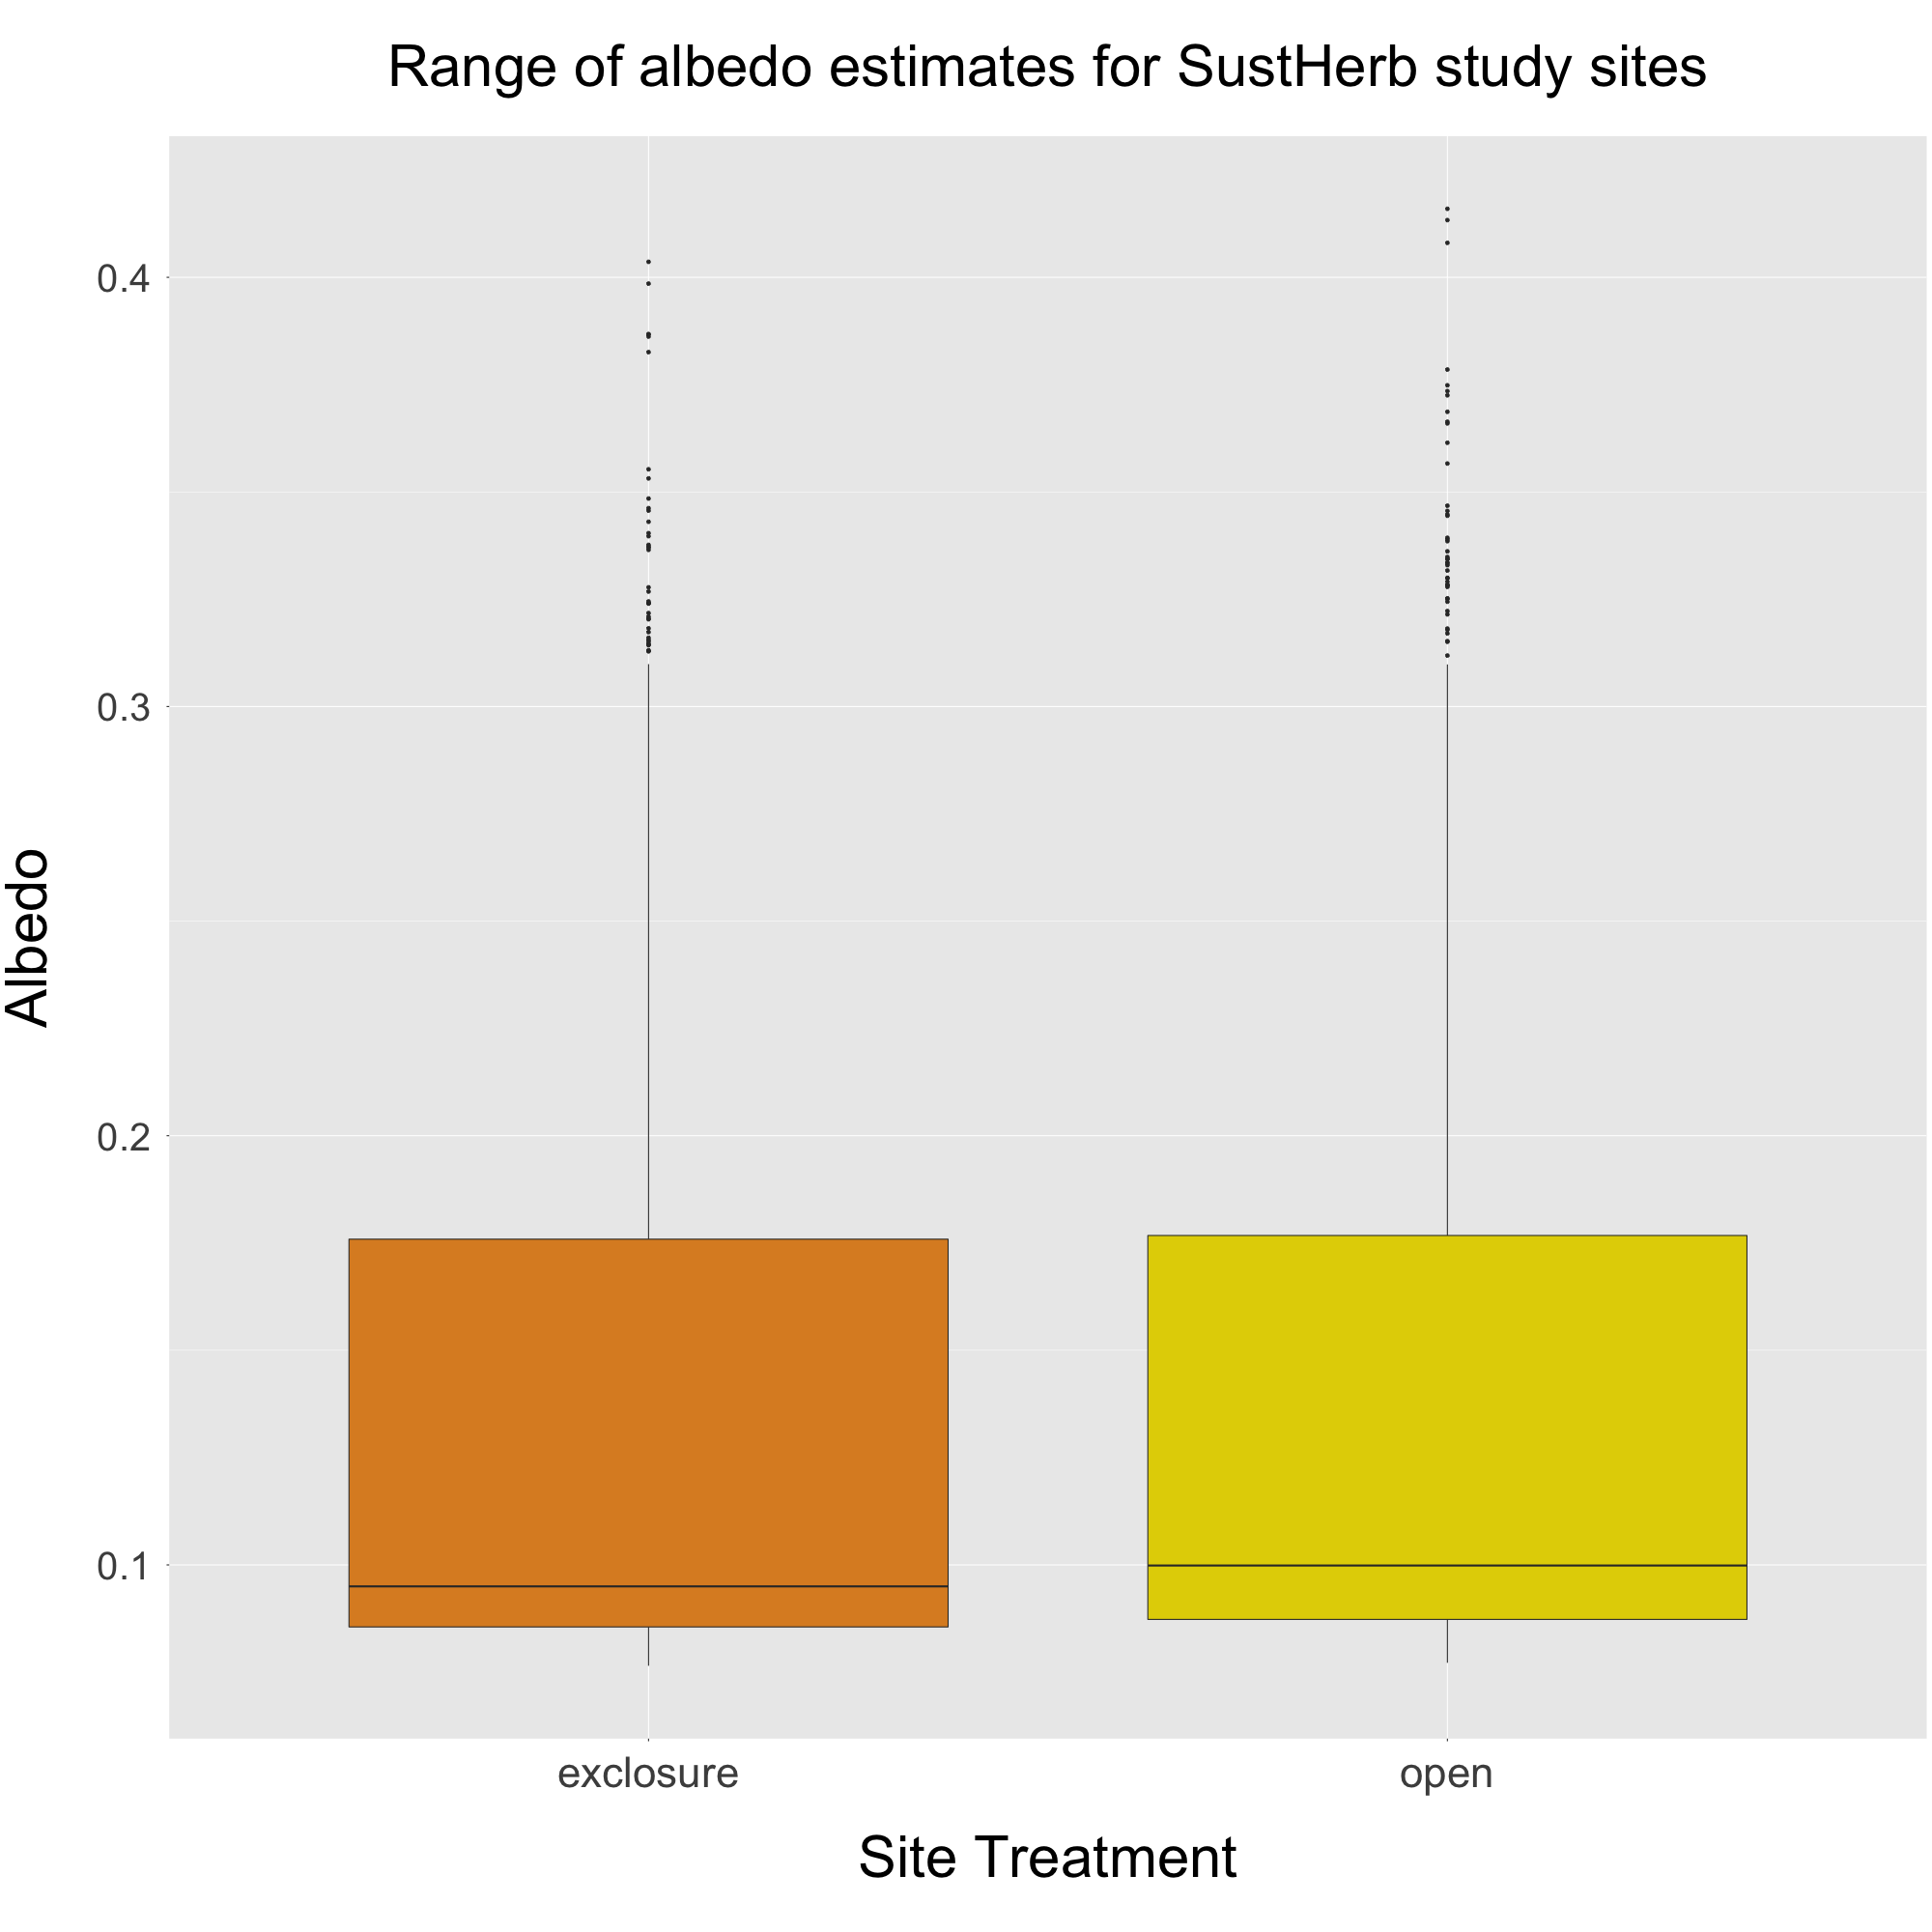
\includegraphics[width=0.8\linewidth]{../../../Approach_3/Output/Albedo_Estimates/albedo_boxplot_approach_3} \end{center}

\begin{center}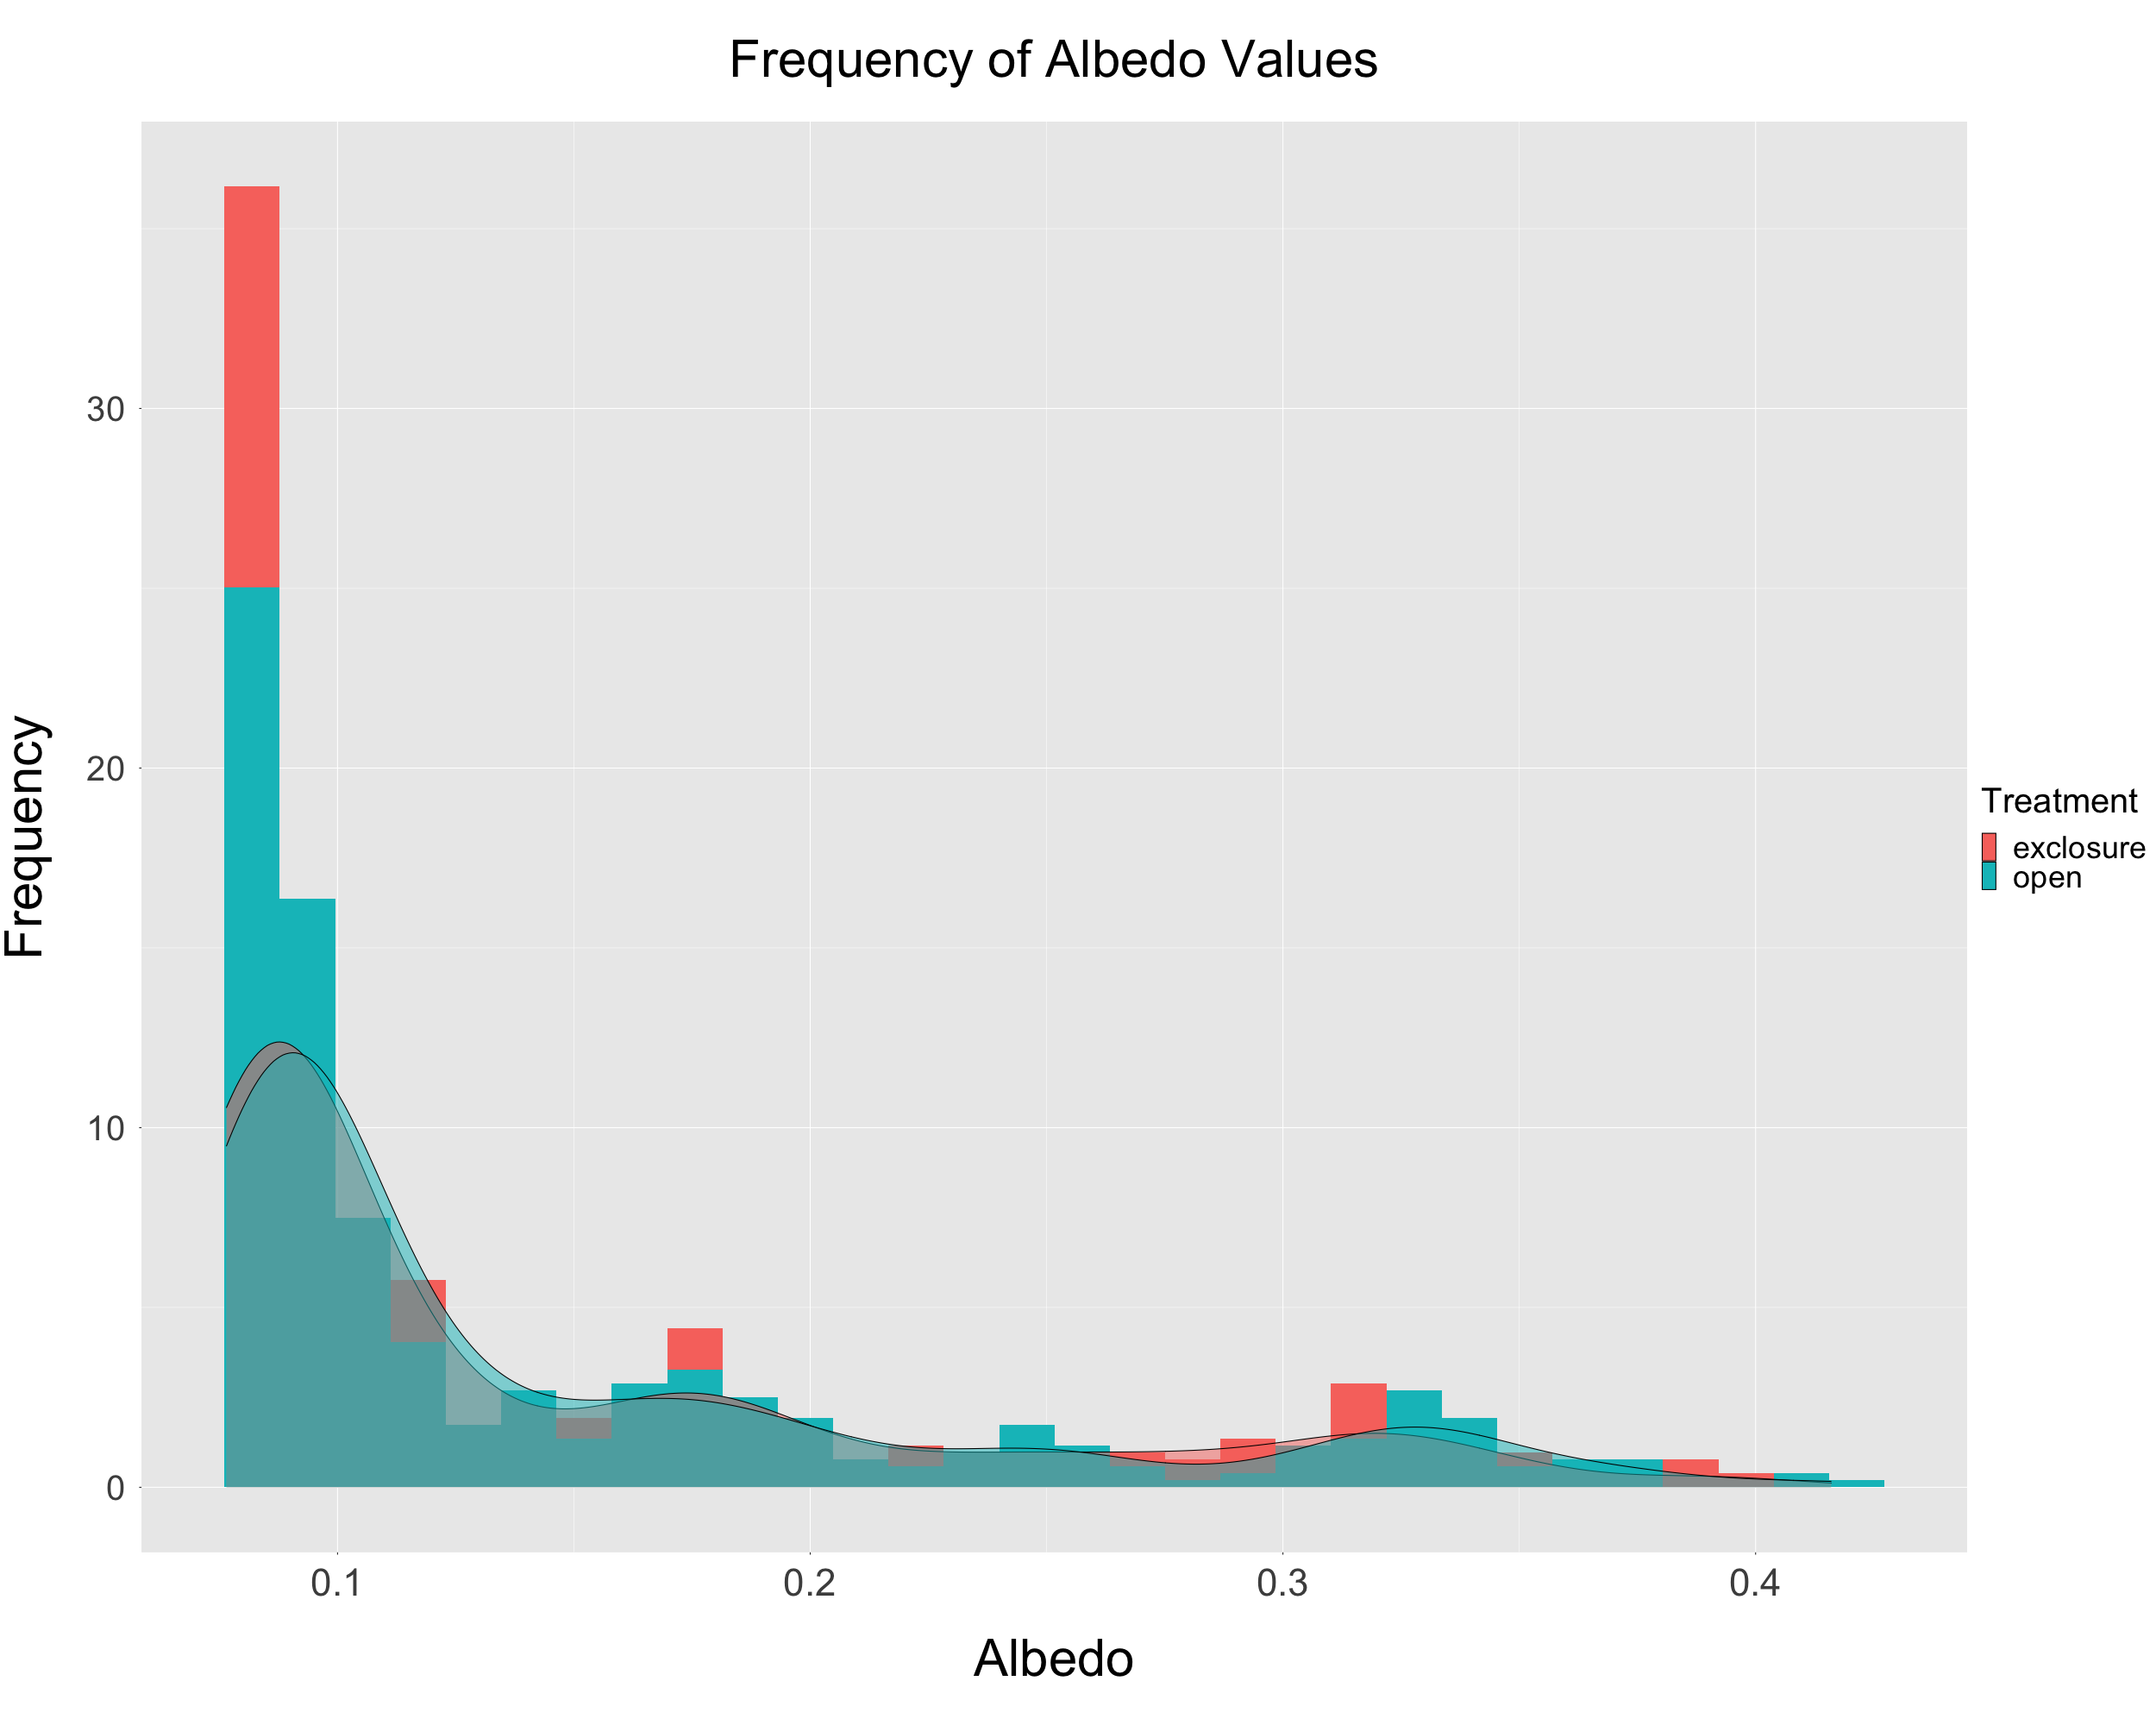
\includegraphics[width=0.8\linewidth]{../../../Approach_3/Output/Albedo_Estimates/albedo_histogram_approach_3} \end{center}

\begin{center}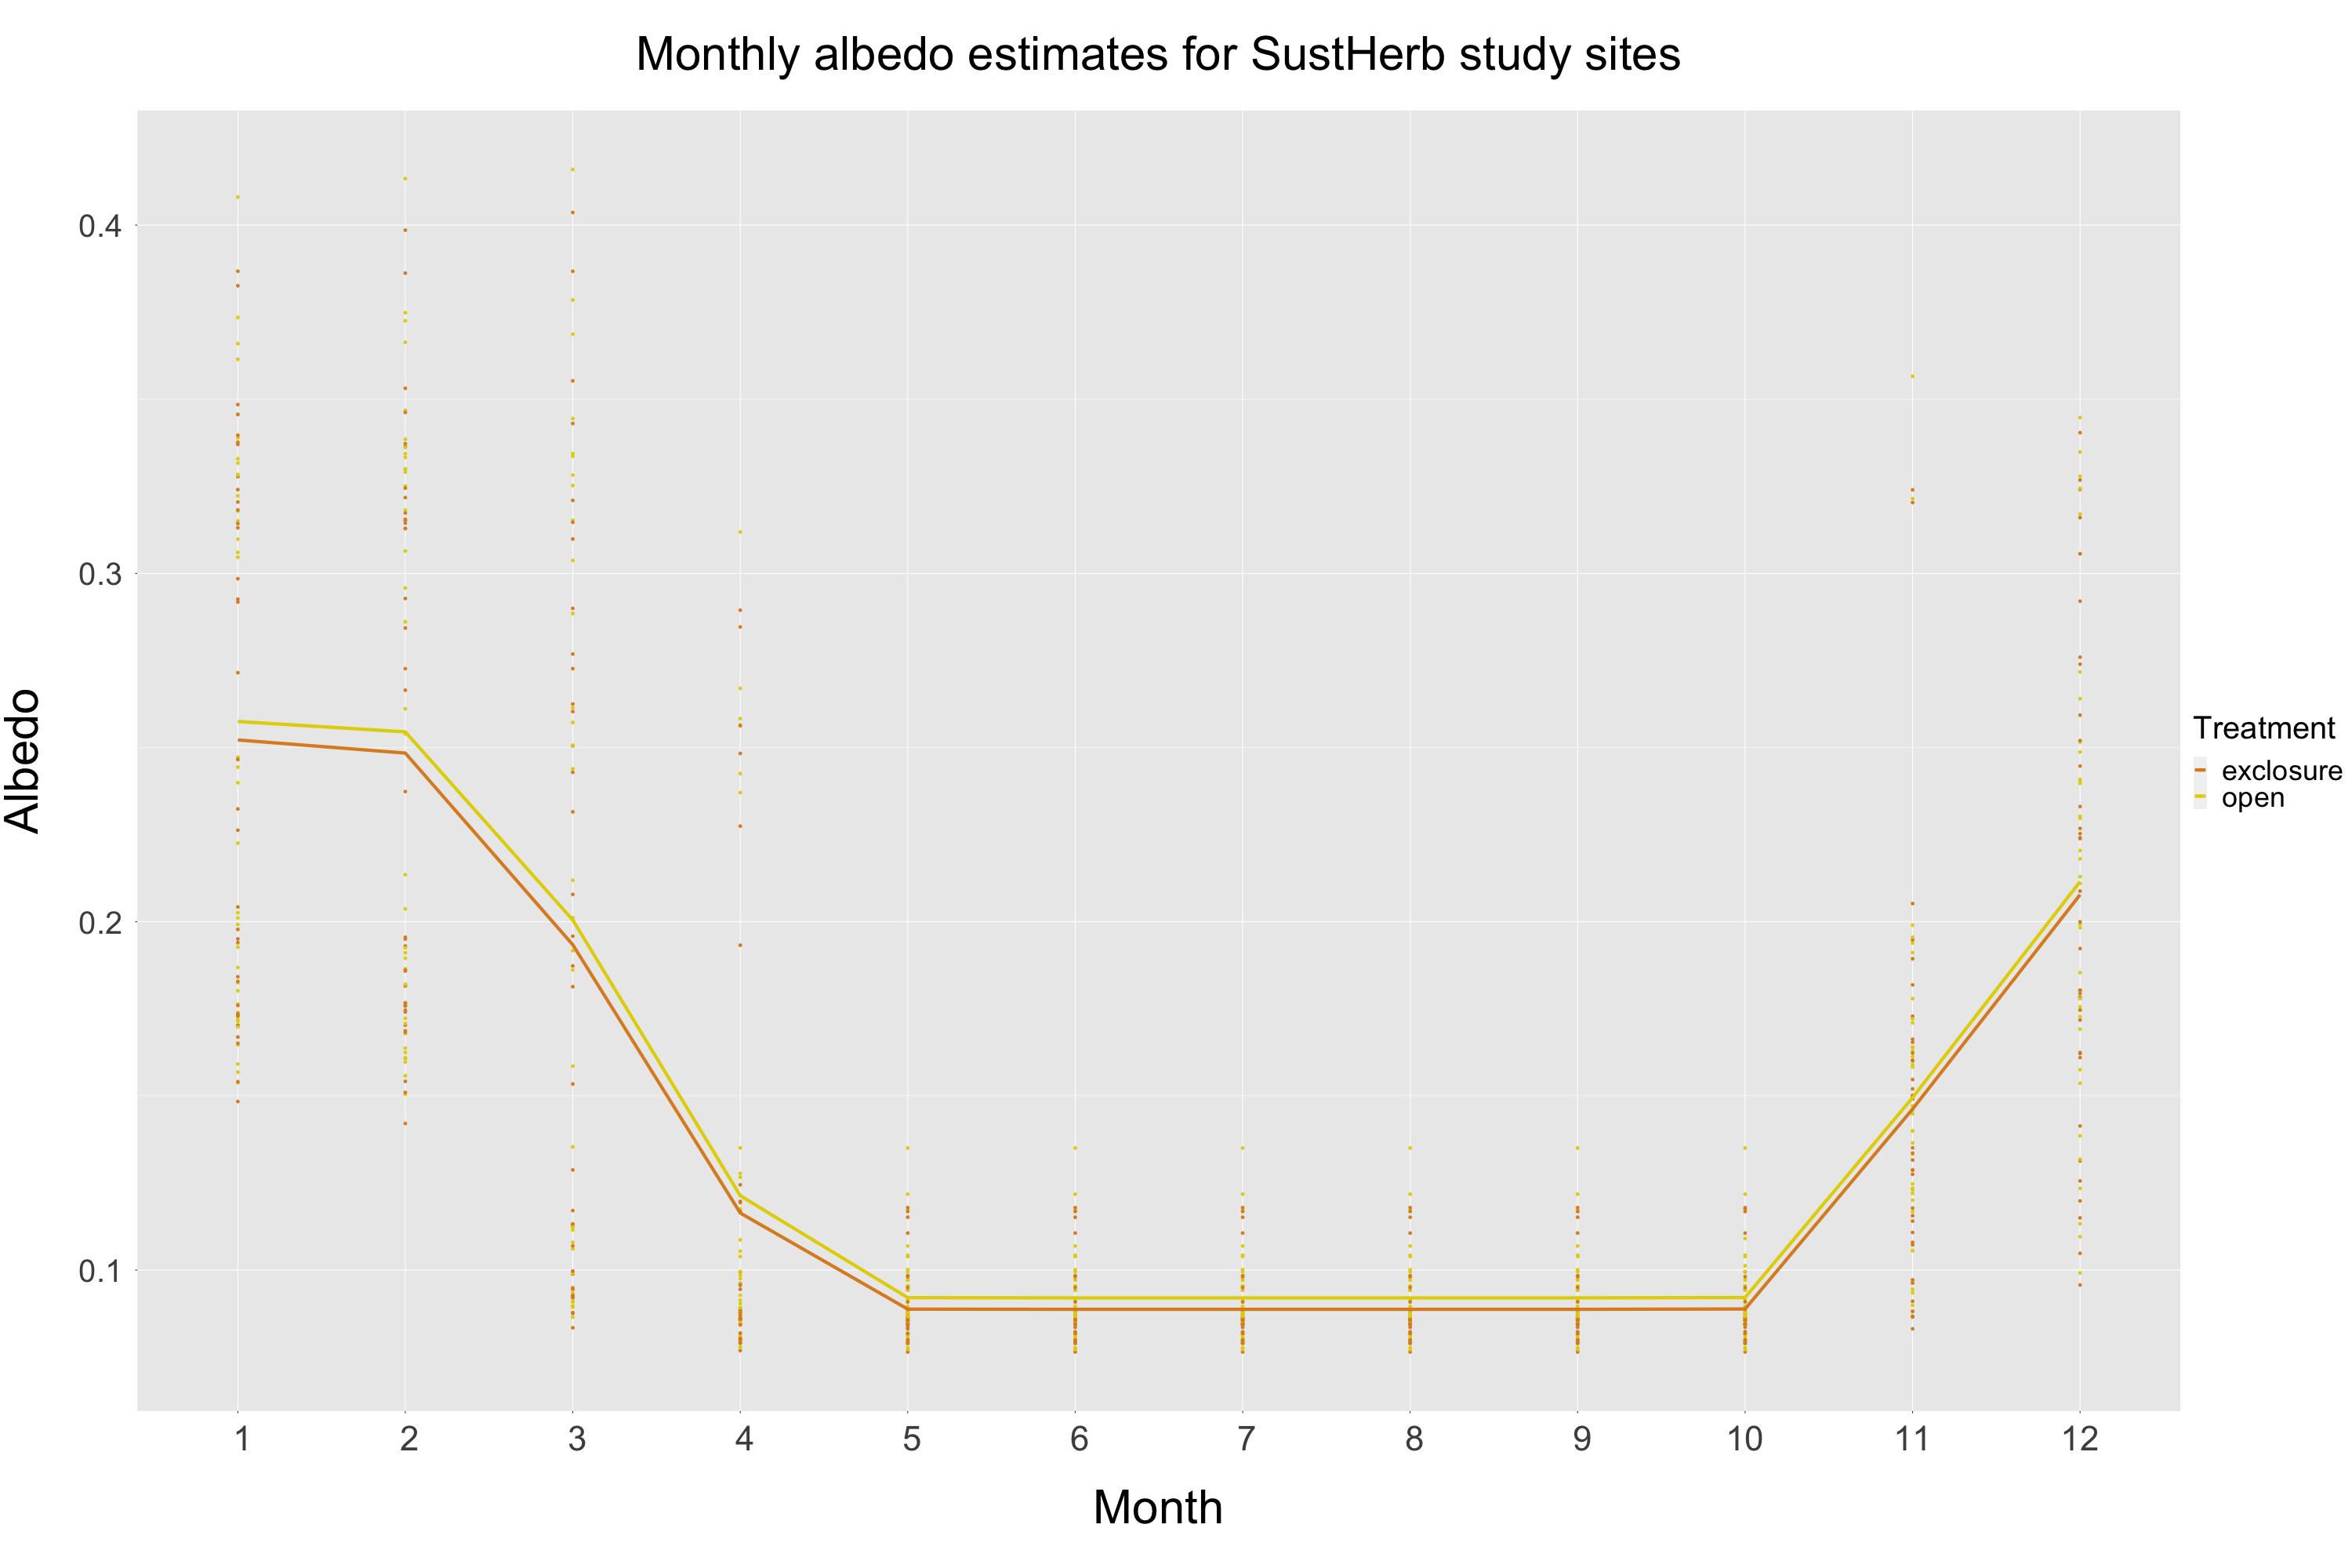
\includegraphics[width=1\linewidth]{../../../Approach_3/Output/Albedo_Estimates/albedo_time_series_approach_3} \end{center}

\begin{center}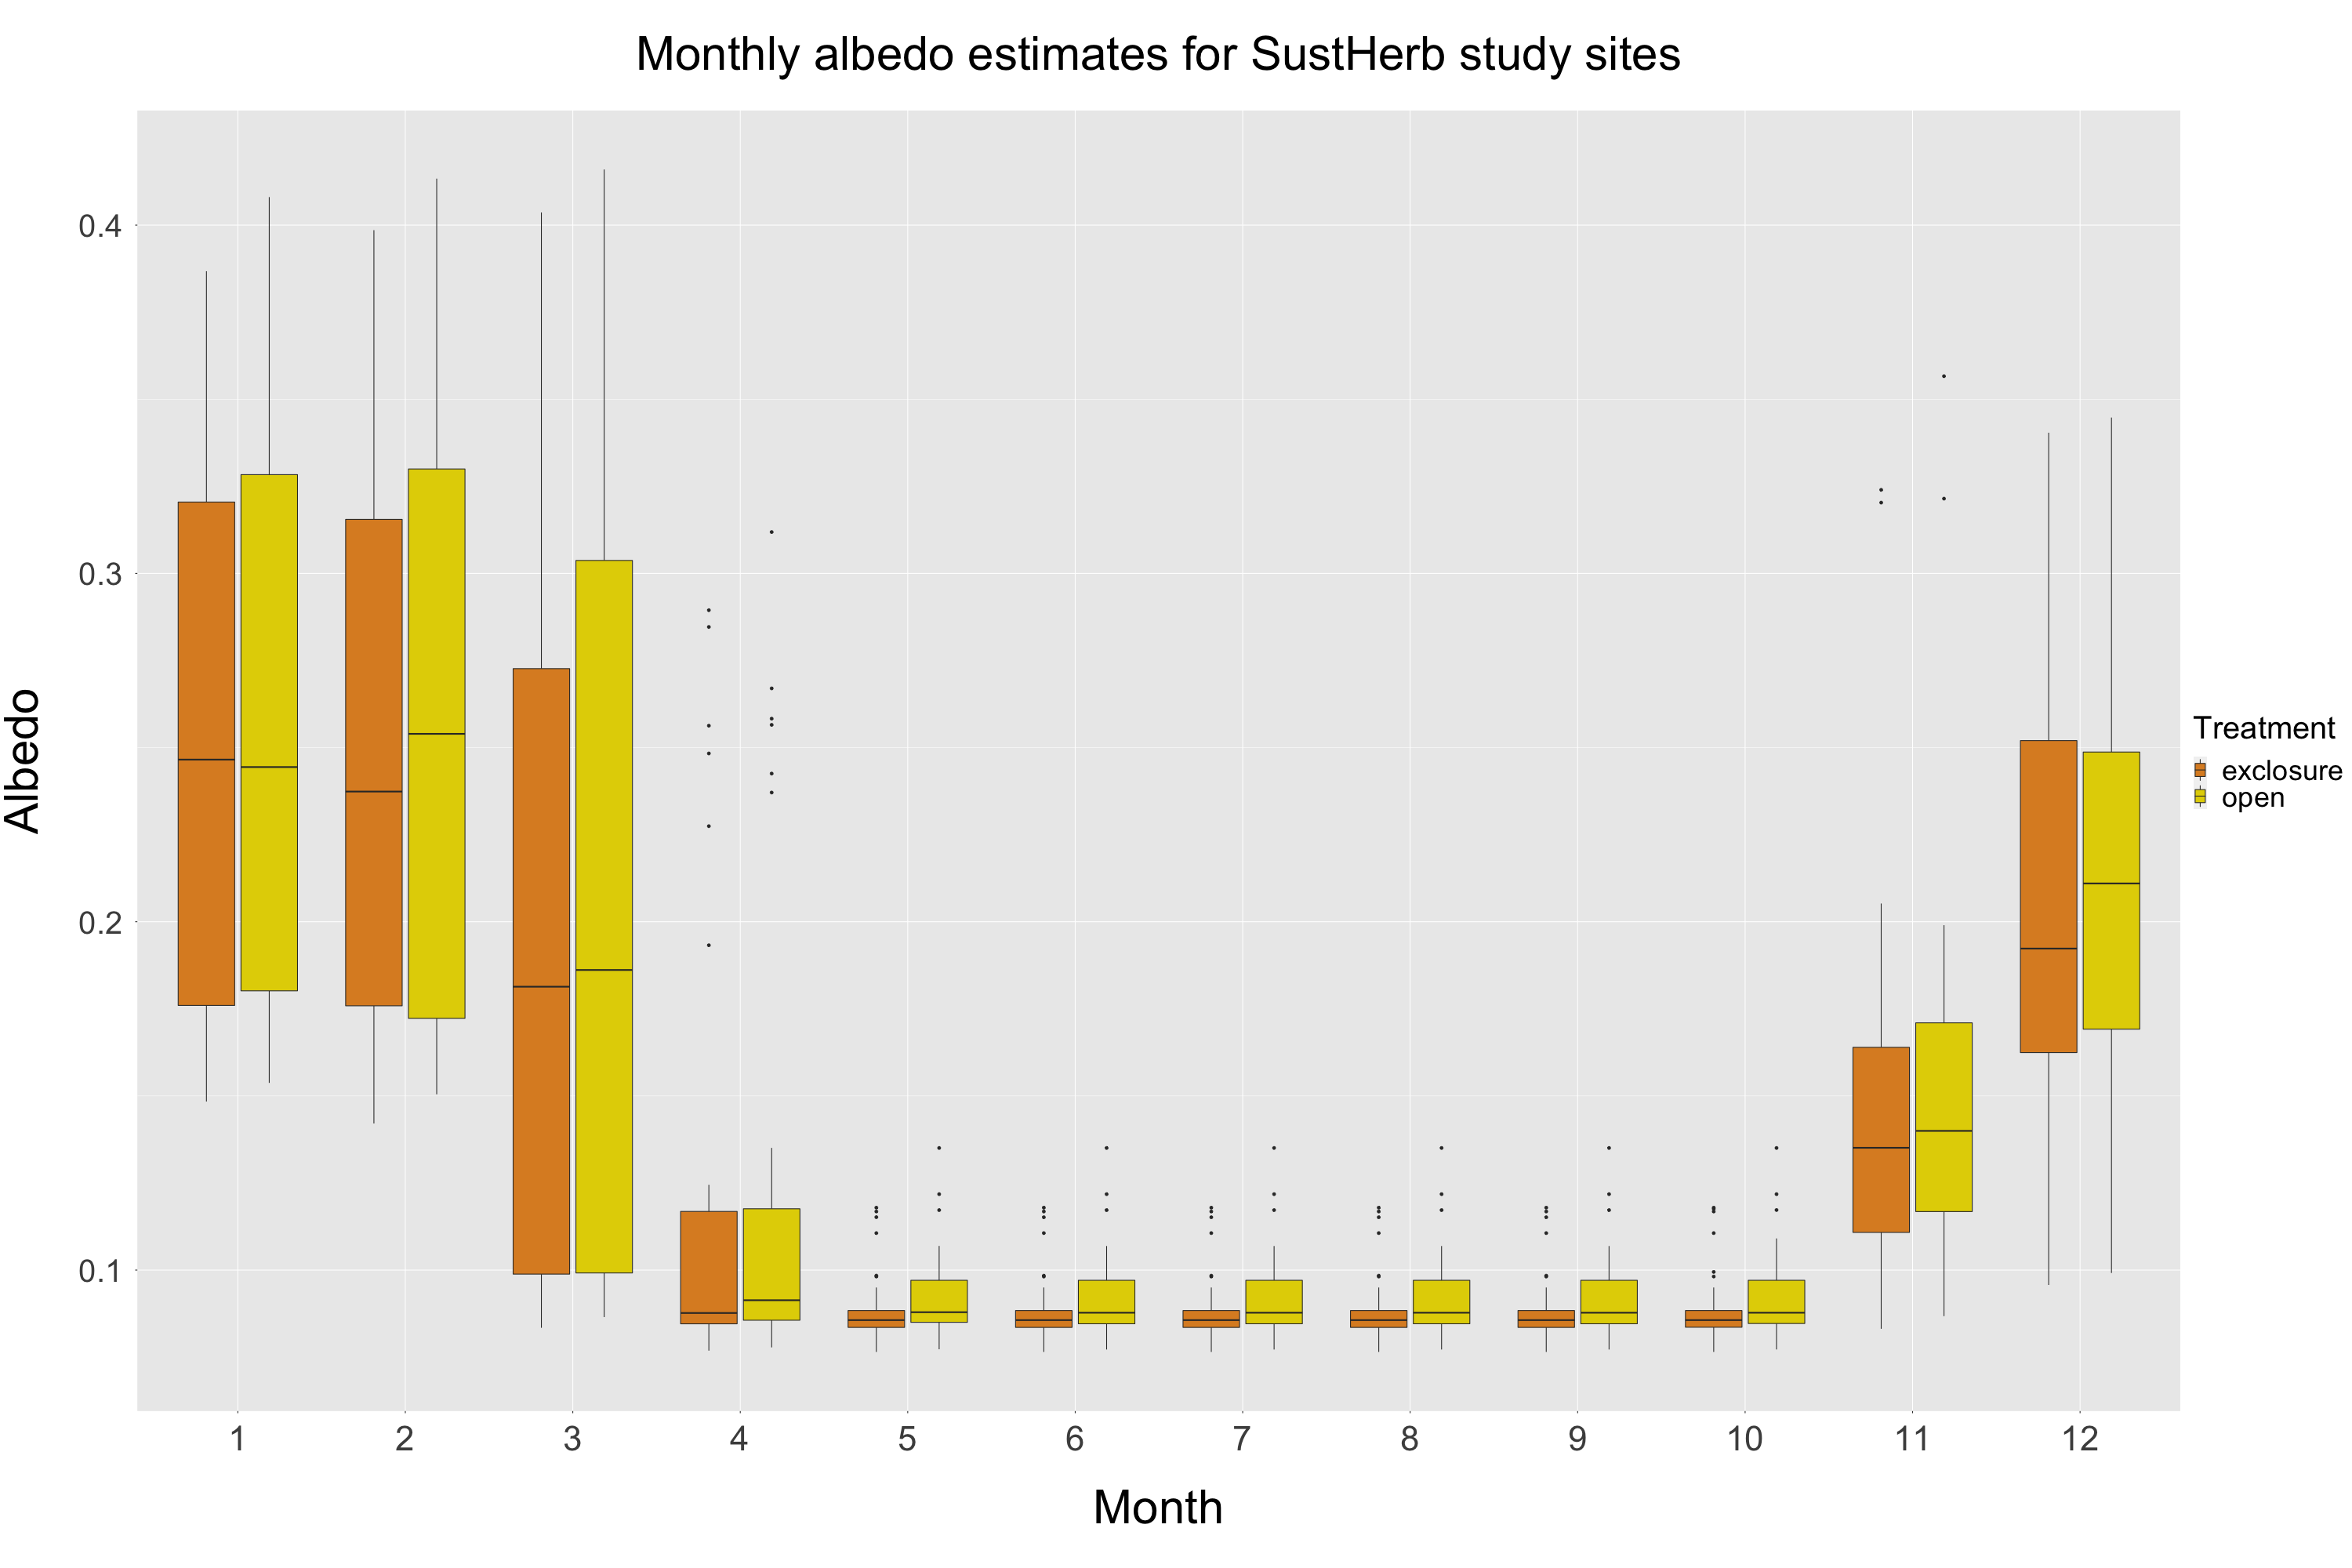
\includegraphics[width=1\linewidth]{../../../Approach_3/Output/Albedo_Estimates/albedo_grouped_boxplot_approach_3} \end{center}

\begin{center}\rule{0.5\linewidth}{0.5pt}\end{center}

\pagebreak

\subsection{Section 2}\label{section-2}

This figure shows an initial attempt at a mixed effects model analysis.

\textbf{Correlation matrix of explanatory variables}: It looks like
`Moose Density' and `Roe Deer Density' are moderately correlated
(\textasciitilde{}0.51).

\begin{center}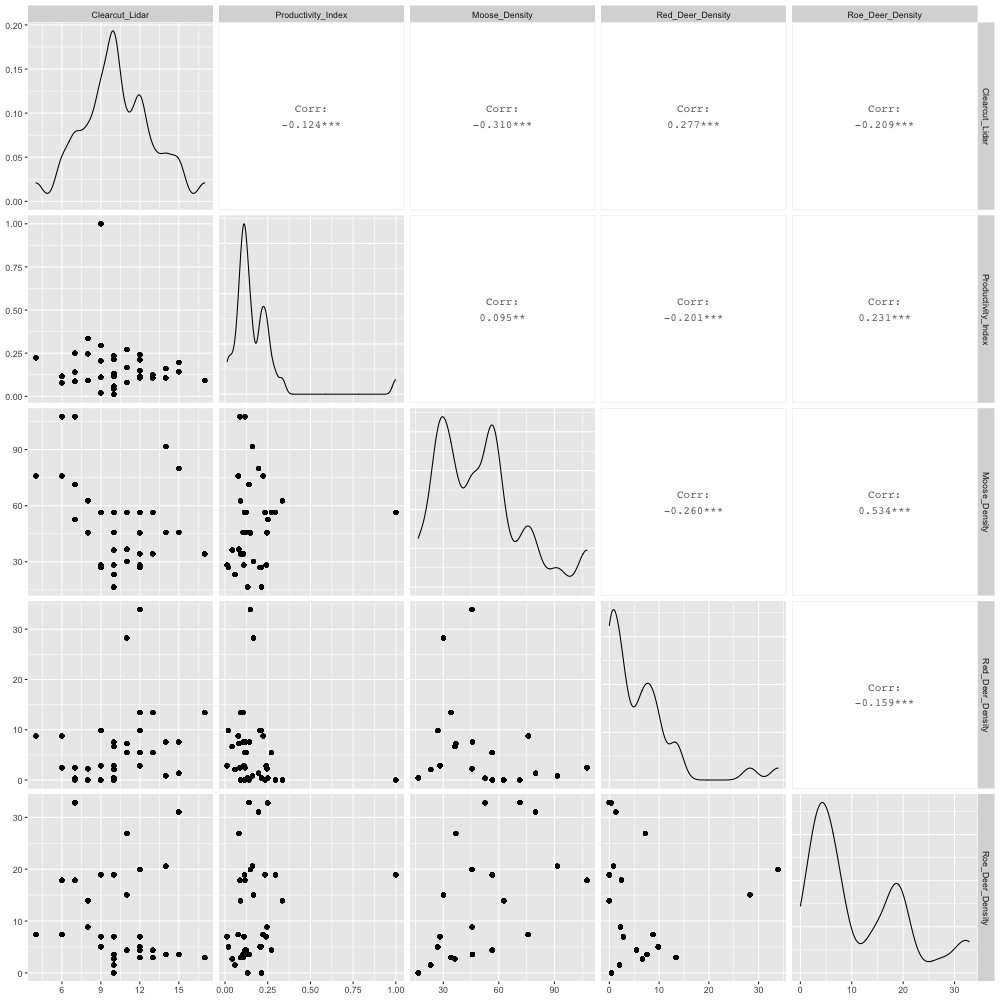
\includegraphics[width=0.8\linewidth]{../../../Approach_3/Output/Analysis/corr_matrix_approach_3} \end{center}

\begin{center}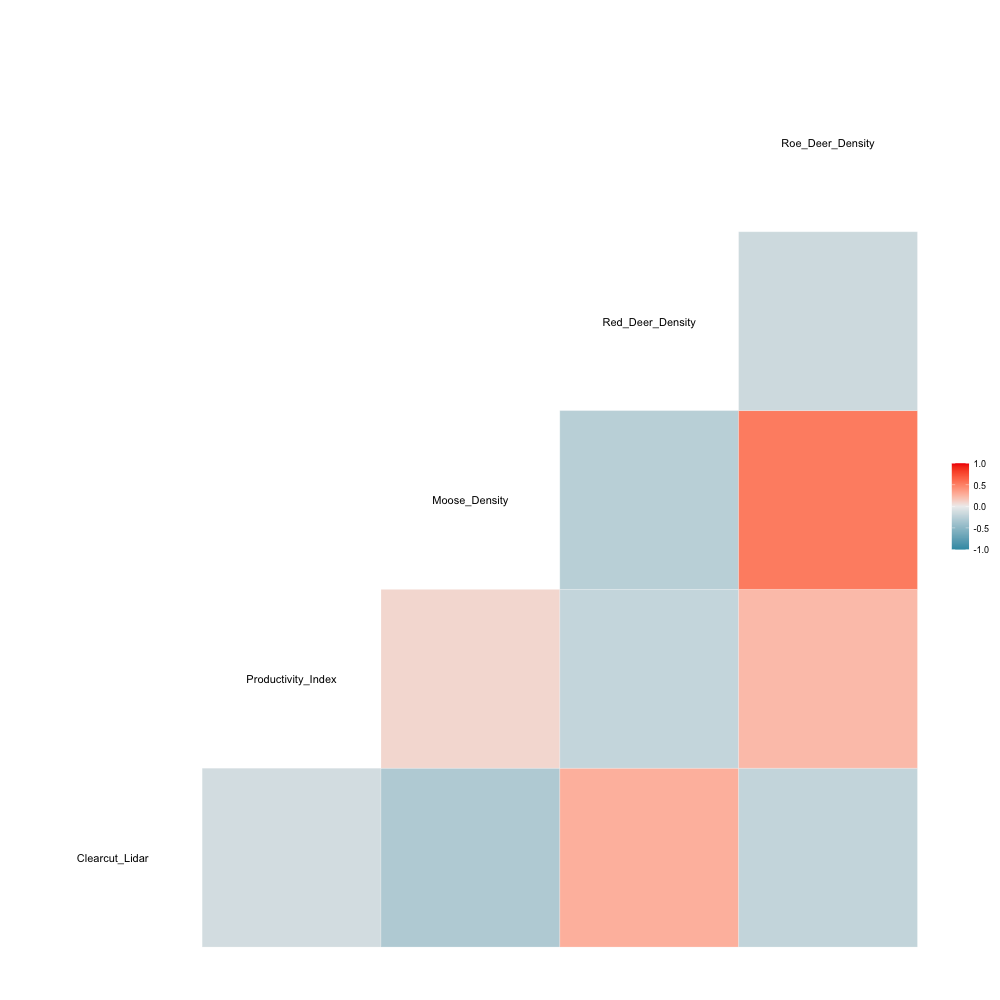
\includegraphics[width=0.8\linewidth]{../../../Approach_3/Output/Analysis/corr_heatmap_approach_3} \end{center}

\textbf{Model in R}: Random effect is month nested under site
(``LocalityName'')

\begin{Shaded}
\begin{Highlighting}[]
\NormalTok{model <-}\StringTok{ }\KeywordTok{lmer}\NormalTok{(Composite_Albedo }\OperatorTok{~}\StringTok{ }\NormalTok{Treatment }\OperatorTok{+}
\StringTok{                      }\NormalTok{Productivity_Index }\OperatorTok{+}
\StringTok{                      }\NormalTok{Clearcut_Lidar }\OperatorTok{+}
\StringTok{                      }\NormalTok{Moose_Density }\OperatorTok{+}
\StringTok{                      }\NormalTok{Red_Deer_Density }\OperatorTok{+}
\StringTok{                      }\NormalTok{Roe_Deer_Density }\OperatorTok{+}
\StringTok{                      }\NormalTok{(}\DecValTok{1} \OperatorTok{|}\StringTok{ }\NormalTok{LocalityName}\OperatorTok{/}\NormalTok{Month),}
              \DataTypeTok{data =}\NormalTok{ model_data)}
\end{Highlighting}
\end{Shaded}

\textbf{Model Output}:

\begin{verbatim}
## Loading required package: Matrix
\end{verbatim}

\begin{verbatim}
## 
## Attaching package: 'lmerTest'
\end{verbatim}

\begin{verbatim}
## The following object is masked from 'package:lme4':
## 
##     lmer
\end{verbatim}

\begin{verbatim}
## The following object is masked from 'package:stats':
## 
##     step
\end{verbatim}

\begin{verbatim}
## Learn more about sjPlot with 'browseVignettes("sjPlot")'.
\end{verbatim}

~

Composite\_Albedo

Predictors

Estimates

CI

p

(Intercept)

0.16940

0.12487~--~0.21393

\textless{}0.001

Treatment {[}open{]}

0.00419

0.00308~--~0.00530

\textless{}0.001

Productivity\_Index

-0.05283

-0.10735~--~0.00170

0.058

Clearcut\_Lidar

-0.00362

-0.00683~--~-0.00041

0.027

Moose\_Density

0.00073

0.00029~--~0.00118

0.001

Red\_Deer\_Density

0.00045

-0.00075~--~0.00165

0.464

Roe\_Deer\_Density

-0.00185

-0.00291~--~-0.00079

0.001

Random Effects

σ2

0.00

τ00 Month:LocalityName

0.01

τ00 LocalityName

0.00

ICC

0.99

N Month

12

N LocalityName

37

Observations

888

Marginal R2 / Conditional R2

0.069 / 0.990

\end{document}
